% Created 2018-11-30 五 13:03
% Intended LaTeX compiler: pdflatex
\documentclass[fontset=none,UTF8,a4paper,zihao=-4]{ctexart}
\usepackage[utf8]{inputenc}
\usepackage[T1]{fontenc}
\usepackage{graphicx}
\usepackage{grffile}
\usepackage{longtable}
\usepackage{wrapfig}
\usepackage{rotating}
\usepackage{amsmath}
\usepackage{textcomp}
\usepackage{amssymb}
\usepackage{capt-of}
\usepackage{hyperref}

\setCJKsansfont{文泉驿微米黑}
\setCJKmonofont{文泉驿微米黑}


%%% 默认使用的latex宏包 %%%
\usepackage{tikz}
\usepackage{CJKulem}
\usepackage{graphicx}

%%% 设置页面边距 %%%
\usepackage[top=2.54cm, bottom=2.54cm, left=3.17cm, right=3.17cm]{geometry} %
\author{yydcnjjw}
\date{\today}
\title{Basic-Zone-Policy3}
\hypersetup{
 pdfauthor={yydcnjjw},
 pdftitle={Basic-Zone-Policy3},
 pdfkeywords={},
 pdfsubject={},
 pdfcreator={Emacs 26.1 (Org mode 9.1.14)}, 
 pdflang={English}}
\begin{document}

\maketitle
\tableofcontents

\begin{figure}[htbp]
\centering
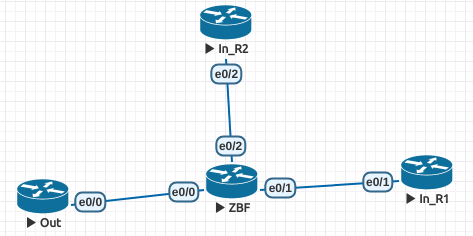
\includegraphics[width=.9\linewidth]{image/experiment/screenshot_2018-11-21_21-18-29.png}
\caption{Topology}
\end{figure}

Configure:
\begin{itemize}
\item Out:
\begin{verbatim}
interface Ethernet0/0
 ip address 202.100.1.1 255.255.255.0
ip route 0.0.0.0 0.0.0.0 202.100.1.10
\end{verbatim}
\item ZBF:
\begin{verbatim}
!
class-map type inspect match-all Self-to-Outside.class
 match access-group name Self-to-Outside
class-map type inspect match-all Self-to-Inside.class
 match access-group name Self-to-Inside
class-map type inspect match-all Inside-to-Self.class
 match access-group name Inside-to-Self
!
policy-map type inspect Self-to-Inside.policy
 class type inspect Self-to-Inside.class
  inspect 
 class class-default
  drop log
policy-map type inspect Outside-to-Self.policy
 class class-default
  drop log
policy-map type inspect Self-to-Outside.policy
 class type inspect Self-to-Outside.class
  inspect 
 class class-default
  drop log
policy-map type inspect Inside-to-Self.policy
 class type inspect Inside-to-Self.class
  inspect 
 class class-default
  drop log
!
zone security Outside
zone security Inside
zone-pair security Self-Outside source self destination Outside
 service-policy type inspect Self-to-Outside.policy
zone-pair security Self-Inside source self destination Inside
 service-policy type inspect Self-to-Inside.policy
zone-pair security Inside-Self source Inside destination self
 service-policy type inspect Inside-to-Self.policy
zone-pair security Outside-Self source Outside destination self
 service-policy type inspect Outside-to-Self.policy
! 
interface Ethernet0/0
 ip address 202.100.1.10 255.255.255.0
 zone-member security Outside
!
interface Ethernet0/1
 ip address 10.1.1.10 255.255.255.0
 zone-member security Inside
!
interface Ethernet0/2
 ip address 172.16.1.10 255.255.255.0
!
ip access-list extended Inside-to-Self
 permit tcp host 10.1.1.1 host 10.1.1.10 eq 22
ip access-list extended Self-to-Inside
 permit tcp host 10.1.1.10 host 10.1.1.1 eq telnet
ip access-list extended Self-to-Outside
 permit icmp host 202.100.1.10 host 202.100.1.1 echo
!
\end{verbatim}
\item In\_R2:
\begin{verbatim}
interface Ethernet0/2
 ip address 172.16.1.1 255.255.255.0
ip route 0.0.0.0 0.0.0.0 172.16.1.10
\end{verbatim}
\item In\_R1:
\begin{verbatim}
interface Ethernet0/1
  ip address 10.1.1.1 255.255.255.0
ip route 0.0.0.0 0.0.0.0 10.1.1.10
\end{verbatim}
\end{itemize}

Test:
ping:
\begin{center}
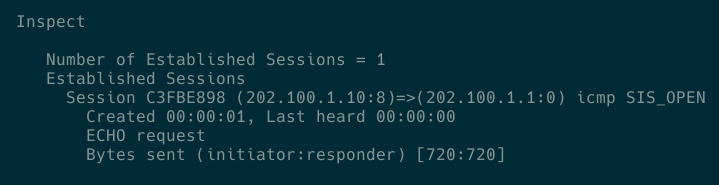
\includegraphics[width=.9\linewidth]{image/experiment/screenshot_2018-11-21_23-07-35.png}
\end{center}
\end{document}